\documentclass[border=10pt]{standalone}

\usepackage{tikz}
\usepackage{tikzsymbols}
\usetikzlibrary{calc,patterns,shapes.geometric}

\def\centerarc[#1](#2)(#3:#4:#5){\draw[#1] ($(#2)+({#5*cos(#3)},{#5*sin(#3)})$) arc (#3:#4:#5);}

\begin{document}
	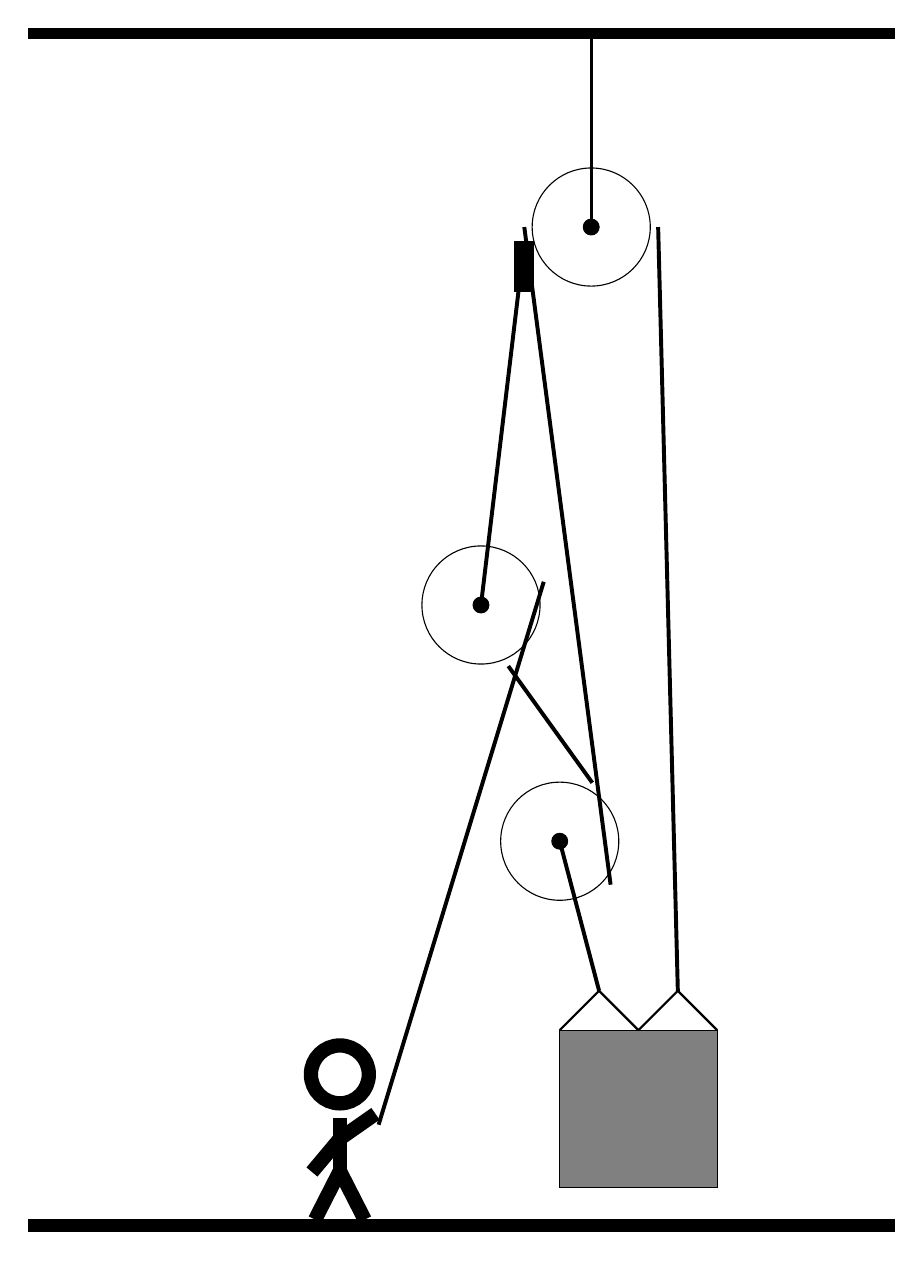
\begin{tikzpicture}
		%%%%% START %%%%%
		\draw[fill=black] (-6, 12) rectangle (5, 12.125);
		
		\draw (-0.25, 4.8) circle (0.75);
		\draw[fill=black] (-0.25, 4.8) circle (0.1);
		
		\draw (0.75, 1.8) circle (0.75);
		\draw[fill=black] (0.75, 1.8) circle (0.1);
		
		\draw (1.15, 9.6) circle (0.75);
		\draw[fill=black] (1.15, 9.6) circle (0.1);
		\draw[very thick] (1.15, 9.6) -- (1.15, 12);
		
		\draw[thick]  (0.75, -0.6) -- (1.25, -0.1) -- (1.75, -0.6) -- (2.25, -0.1) -- (2.75, -0.6);
		\draw[fill=black!50] (0.75, -0.6) rectangle (2.75, -2.6);
		
		\draw[line width=0.5mm] (-0.25, 4.8) -- (0.3, 9.4);
		\draw[line width=0.5mm, fill=black](0.2, 8.8) rectangle (0.4, 9.4);
		\draw[line width=0.5mm] (-1.55, -1.8) -- (0.547, 5.095);
		\centerarc[line width=0.5mm](-0.25, 4.8)(-20:170:0.85);
		\draw[line width=0.5mm] (0.097, 4.024) -- (1.164, 2.542);
		\centerarc[line width=0.5mm](0.75, 1.8)(160:380:0.85);
		\draw[line width=0.5mm] (1.396, 1.248) -- (0.3, 9.6);
		\draw[line width=0.5mm](0.75, 1.8) -- (1.25, -0.1);
		\centerarc[line width=0.5mm](1.15, 9.6)(0:180:0.85);
		\draw[line width=0.5mm] (2.0, 9.6) -- (2.25, -0.1);
		
		\node at (-2, -1.9) {\Strichmaxerl[10][50][35]};
		
		\draw[fill=black] (-6, -3) rectangle (5, -3.15);
		%%%%% END %%%%%
	\end{tikzpicture}
\end{document}